\section{定义Kernel}
到目前为止,在本书中,我们的代码示例已经使用 C++ lambda 表达式表示Kernel。 
Lambda 表达式是一种在使用时表示Kernel的简洁而方便的方法,但它们并不是在 SYCL 中表示Kernel的唯一方法。 
在本章中,我们将详细探讨定义Kernel的各种方法,帮助我们选择最适合我们的 C++ 编码需求的Kernel形式。

本章解释并比较了表示Kernel的三种方法:

\begin{itemize}
	\item Lambda 表达式。

	\item 命名函数对象(Functor)。

	\item 通过与通过其他语言或API 创建的Kernel的互操作性。 本章简要介绍了该主题,第 20 章更详细地介绍了该主题。
\end{itemize}

本章最后讨论了如何显式操作Kernel包中的Kernel来查询Kernel属性并控制何时以及如何编译Kernel。


\subsection{为什么用三种方式来表示Kernel?}
\begin{figure}[H]
	\centering
	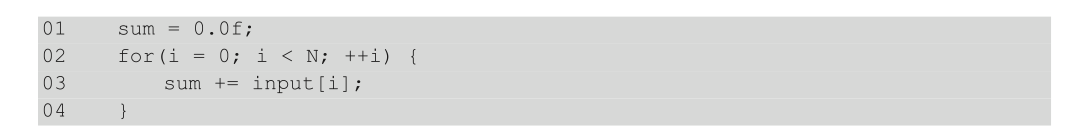
\includegraphics[width=0.9\textwidth]{figs/F10.1.png}
	\caption{\textit{表示 Kernel 的三种方式 }}
\end{figure}

在深入讨论细节之前,我们首先总结一下为什么有三种定义Kernel的方法以及每种方法的优缺点。 
图 10-1 给出了一个有用的总结。

请记住,Kernel用于表示计算单元,并且Kernel的许多实例通常会在加速器上并行执行。 
SYCL 支持多种方式来表达Kernel,以自然、无缝地集成到具有不同编码风格的代码库中,同时还能在各种加速器类型上高效执行。

\subsection{作为 Lambda 表达式的Kernel}
C++ lambda 表达式,也称为匿名函数对象、未命名函数对象、闭包或简称 lambda,是在使用Kernel时表达Kernel的便捷方法。 
本节介绍如何将Kernel表示为 C++ lambda 表达式。 
这扩展了第 1 章中 C++ lambda 表达式的介绍性复习,其中包括一些带有输出的基本编码示例。

C++ lambda 表达式非常强大并且具有表达语法,
但在 SYCL 中表达Kernel时,仅需要(并支持)完整 C++ lambda 表达式语法的特定子集。

\subsubsection{Kernel Lambda 表达式的元素}
\begin{figure}[H]
	\centering
	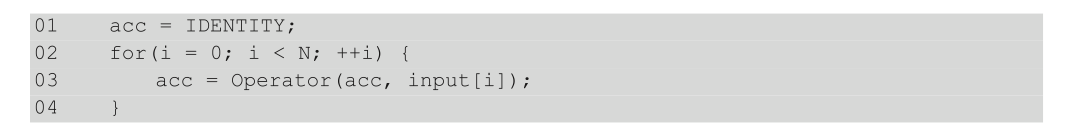
\includegraphics[width=0.9\textwidth]{figs/F10.2.png}
	\caption{\textit{使用 lambda 表达式定义的简单Kernel }}
\end{figure}

图 10-2 显示了一个用典型 lambda 表达式编写的简单Kernel——本书到目前为止的代码示例都使用了这种语法。

\begin{figure}[H]
	\centering
	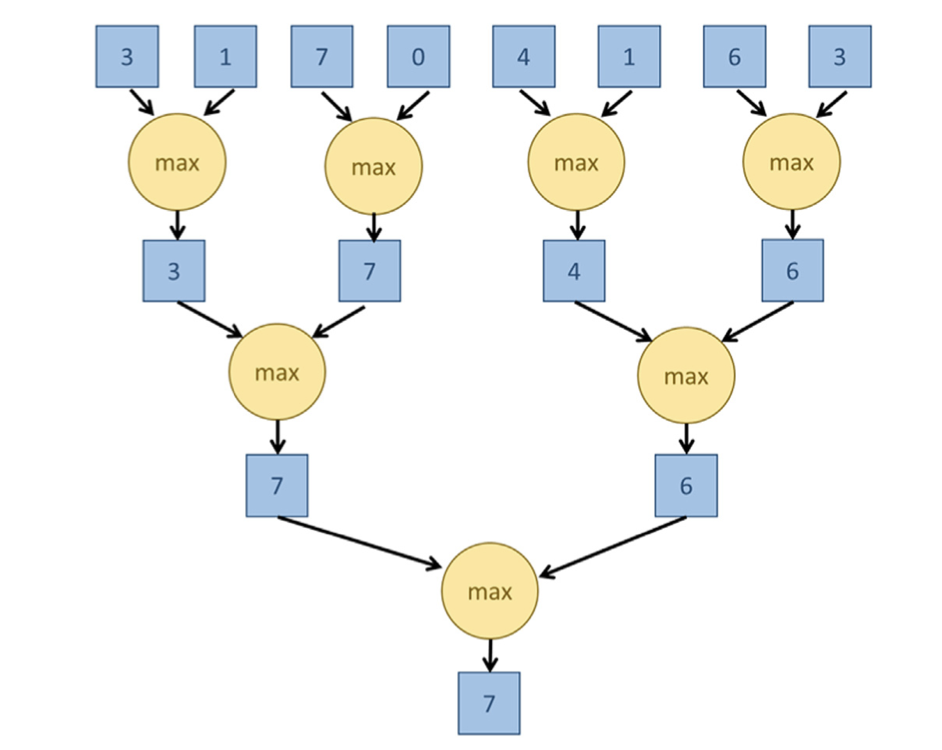
\includegraphics[width=0.9\textwidth]{figs/F10.3.png}
	\caption{\textit{Kernel lambda 表达式的更多元素,包括可选元素 }}
\end{figure}

图 10-3 中的插图显示了可与Kernel一起使用的 lambda 表达式的元素,但其中许多元素并不典型。 
在大多数情况下,lambda 默认值就足够了,因此典型的Kernel lambda 表达式看起来更像图 10-2 中的 lambda 表达式,
而不是图 10-3 中更复杂的 lambda 表达式。

\begin{enumerate}
	\item lambda 表达式的第一部分描述 lambda 捕获。 
	从周围范围捕获变量使其可以在 lambda 表达式中使用,而无需将其作为参数显式传递给 lambda 表达式。

	C++ lambda 表达式支持通过复制或创建对变量的引用来捕获变量,
	但对于Kernel lambda 表达式,只能通过复制来捕获变量。 
	一般做法是简单地使用默认捕获模式 [=],该模式按值隐式捕获所有变量,
	尽管也可以在逗号分隔的捕获列表中显式命名每个捕获的变量。 
	Kernel中使用的任何未按值捕获的变量都将导致编译时错误。 
	请注意,根据 C++ 标准,全局变量不会被 lambda 表达式捕获。

	\item lambda 表达式的第二部分描述传递给 lambda 表达式的参数,就像传递给命名函数的参数一样。 
	对于Kernel lambda 表达式,该参数取决于Kernel的调用方式并标识并行执行空间中工作项的索引。 
	有关各种并行执行空间以及如何识别每个执行空间中工作项的索引的更多详细信息,请参阅第 4 章。

	\item lambda 表达式的最后一部分定义函数体。 
	对于Kernel lambda 表达式,函数体描述了应在并行执行空间中的每个索引处执行的操作。

	lambda 表达式还有其他部分,但它们要么是可选的、不经常使用的,要么不受 SYCL 2020 支持:

	\item SYCL 2020 没有定义任何说明符(例如 mutable),因此示例代码中没有显示任何说明符。

	\item 支持异常规范,但如果提供,则必须为 noexcept,因为Kernel不支持异常。

	\item 支持 Lambda 属性,可用于控制Kernel的编译方式。 
	例如,reqd\_work\_group\_size 属性可用于要求Kernel的特定工作组大小,
	而 device\_has 属性可用于要求Kernel的特定设备方面。 
	第 12 章包含有关使用属性和方面进行Kernel专业化的更多信息。

	\item 可以指定返回类型,但如果提供则必须为 void,因为Kernel不支持非 void 返回类型。
\end{enumerate}

\begin{remark}[LAMBDA 捕获:隐式还是显式?]
由于可能存在的悬空指针问题,某些 C++ 样式指南建议不要对 lambda 表达式进行隐式(或默认)捕获,
尤其是当 lambda 表达式跨越范围边界时。
当使用 lambda 表示Kernel时,可能会出现同样的问题,因为Kernel lambda 在设备上异步执行,与主机代码分开。

由于隐式捕获有用且简洁,因此它是 SYCL Kernel的常见做法,
也是我们在本书中使用的约定,但最终由我们决定是选择隐式捕获的简洁性还是显式捕获的清晰性。
\end{remark}

\subsubsection{识别Kernel Lambda 表达式}
\begin{figure}[H]
	\centering
	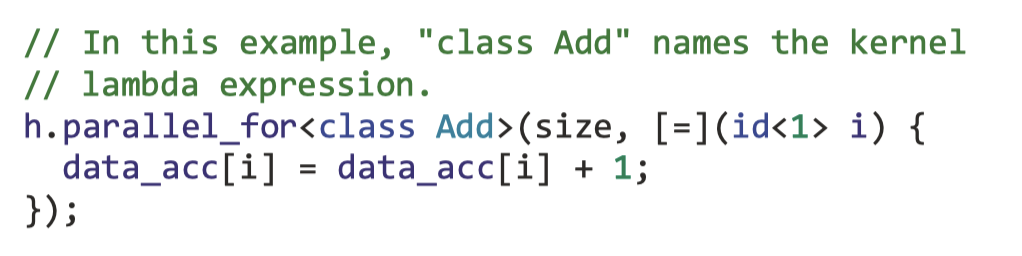
\includegraphics[width=0.9\textwidth]{figs/F10.4.png}
	\caption{\textit{识别Kernel lambda 表达式 }}
\end{figure}

当将Kernel编写为 lambda 表达式时,在某些情况下还必须提供一个元素:因为 lambda 表达式是匿名的,
所以有时 SYCL 需要显式Kernel名称模板参数来唯一标识编写为 lambda 表达式的Kernel。

命名Kernel lambda 表达式是主机代码编译器在由单独的设备代码编译器编译Kernel时识别要调用哪个Kernel的一种方式。 
命名Kernel lambda 还可以对已编译Kernel进行运行时自省或按名称构建Kernel,如图 10-9 所示。

\begin{figure}[H]
	\centering
	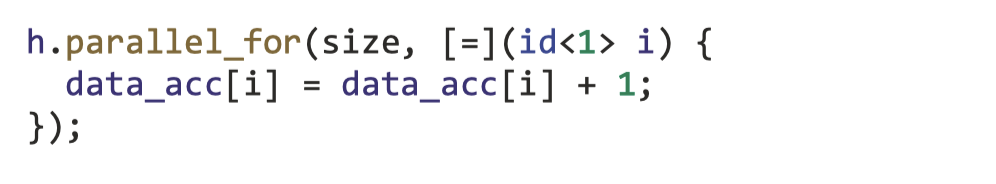
\includegraphics[width=0.9\textwidth]{figs/F10.5.png}
	\caption{\textit{使用未命名的Kernel lambda 表达式 }}
\end{figure}

为了在不需要Kernel名称模板参数时支持更简洁的代码,对于大多数 SYCL 2020 编译器来说,Kernel名称模板参数是可选的。 
当不需要Kernel名称模板参数时,我们的代码可以更加紧凑,如图10-5所示。

由于大多数情况下不需要 lambda 表达式的Kernel名称模板参数,
因此我们通常可以从未命名的 lambda 开始,仅在需要Kernel名称模板参数的特定情况下添加Kernel名称。

\begin{remark}
	当不需要Kernel名称模板参数时,最好使用未命名的Kernel lambda 来减少冗长。
\end{remark}

\subsection{Kernel作为命名函数对象}
命名函数对象,也称为Functor,是 C++ 中的一种既定模式,允许在维护定义良好的接口的同时对任意数据集合进行操作。 
当用于表示Kernel时,命名函数对象的成员变量定义Kernel可以操作的状态,
并且为并行执行空间中的每个工作项调用重载函数调用operator()。

命名函数对象需要比 lambda 表达式更多的代码来表达Kernel,但额外的冗长提供了更多的控制和附加功能。 
例如,分析和优化表示为命名函数对象的Kernel可能会更容易,
因为Kernel使用的任何缓冲区和数据值都必须显式传递给Kernel,而不是由 lambda 表达式自动捕获。

表示为命名函数对象的Kernel也可能更容易调试、更容易重用,并且它们可以作为单独的头文件或库的一部分提供。

最后,因为命名函数对象就像任何其他 C++ 类一样,所以可以模板化表示为命名函数对象的Kernel。 
C++20 添加了模板化 lambda 表达式,但基于 C++17 的 SYCL 2020 中的Kernel不支持模板化 lambda 表达式。

\subsubsection{Kernel命名函数对象的元素}
\begin{figure}[H]
	\centering
	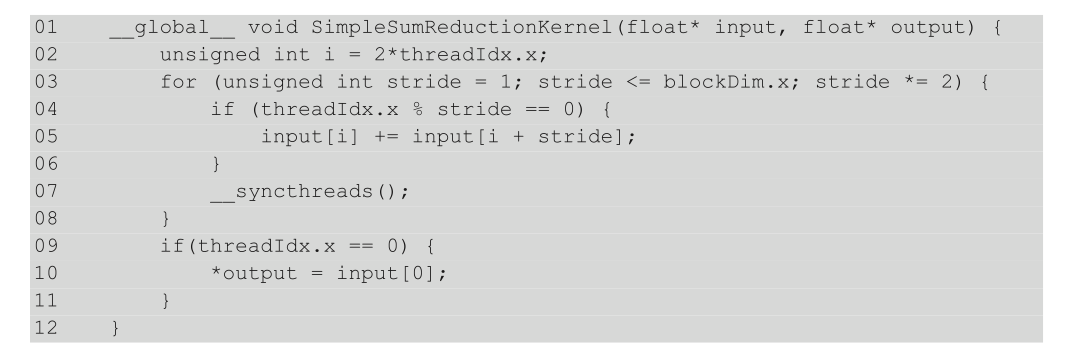
\includegraphics[width=0.9\textwidth]{figs/F10.6.png}
	\caption{\textit{Kernel作为命名函数对象 }}
\end{figure}

图 10-6 中的代码演示了表示为命名函数对象的Kernel的典型用法。 
在这个例子中,Kernel的参数被传递给类构造函数,而Kernel本身则在重载函数调用operator()中。

当Kernel表示为命名函数对象时,命名函数对象类型必须遵循 SYCL 2020 规则才能设备可复制。 
通俗地说,这意味着命名函数对象可以逐字节安全地复制,
从而使命名函数对象的成员变量能够传递到设备上执行的Kernel代码并由其访问。 
任何可普通复制的 C++ 类型都是隐式设备可复制的。

重载函数调用operator()的参数取决于Kernel的启动方式,就像用lambda表达式表示的Kernel一样。

\begin{figure}[H]
	\centering
	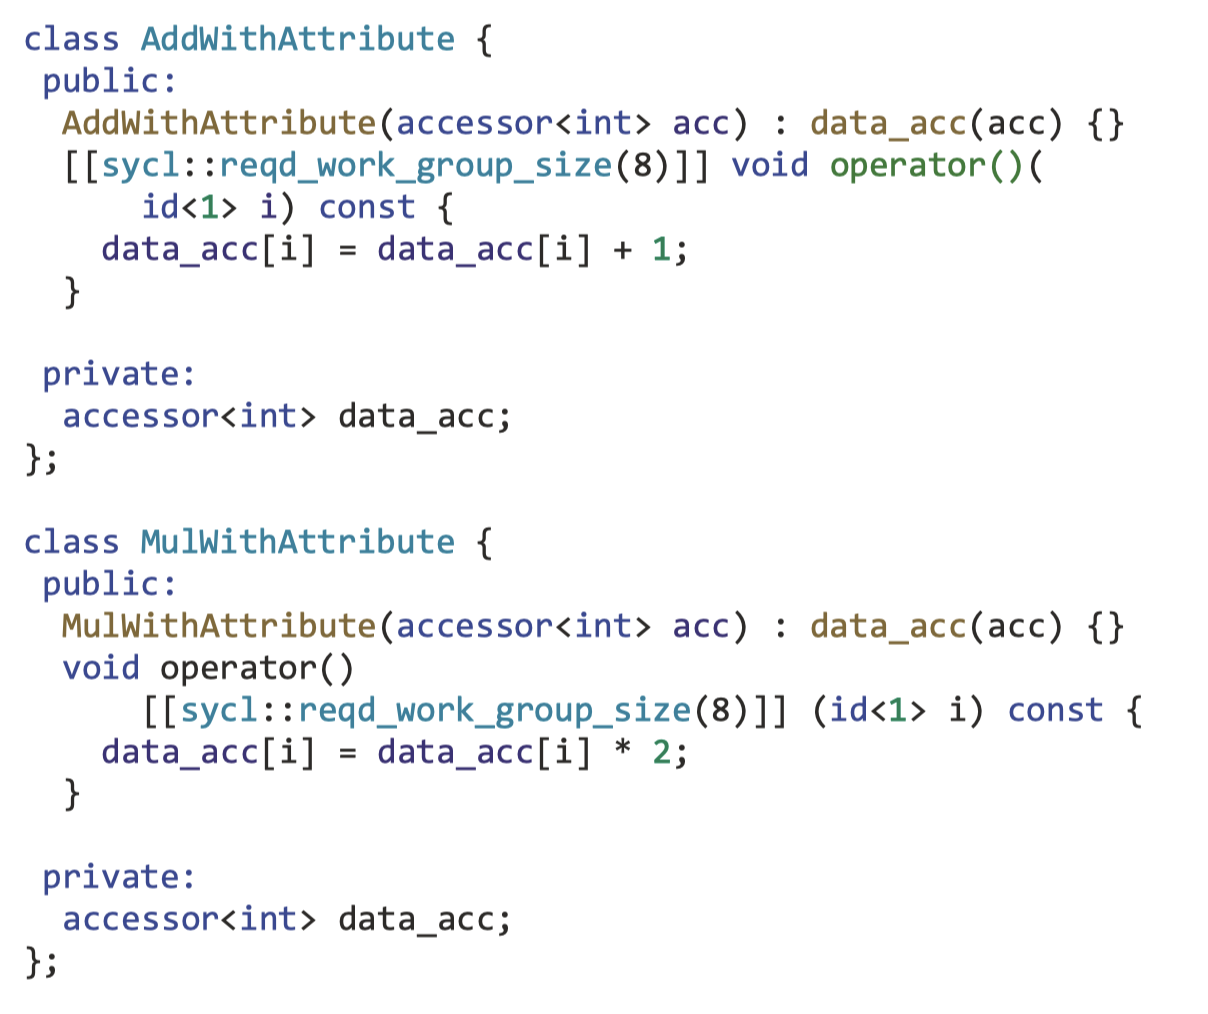
\includegraphics[width=0.9\textwidth]{figs/F10.7.png}
	\caption{\textit{将可选属性与命名函数对象一起使用 }}
\end{figure}

图 10-7 中的代码显示了如何在定义为命名函数对象的Kernel上使用可选的Kernel属性,
例如 reqd\_work\_group\_size 属性。 
当Kernel被定义为命名函数对象时,可选Kernel属性有两个有效位置。 
这与编写为 lambda 表达式的Kernel不同,其中可选Kernel属性只有一个位置有效。

由于所有函数对象都是命名的,因此即使函数对象是模板化的,
主机代码编译器也可以使用函数对象类型来识别设备代码编译器生成的Kernel代码。 
不需要额外的Kernel名称模板参数来命名Kernel函数对象。

\subsection{Kernel包中的Kernel}
我们应该注意的与 SYCL Kernel相关的最后一个主题涉及 SYCL Kernel对象和 SYCL Kernel包。 
典型的应用程序开发不需要了解Kernel对象和Kernel包,但在某些情况下对于调整应用程序性能很有用。 
了解Kernel对象和Kernel包还可以帮助理解 SYCL 实现如何组织和管理Kernel。

SYCL Kernel包是应用程序使用的 SYCL Kernel或 SYCL 函数的容器。 
应用程序中Kernel包的数量取决于特定的 SYCL 编译器。 
一些应用程序可能只有一个Kernel包,即使它们有多个Kernel,而其他应用程序可能有多个Kernel包,即使它们只有几个Kernel。

SYCL Kernel包及其包含的Kernel或函数可以处于以下三种状态之一:

\begin{itemize}
	\item \textbf{输入状态}:此状态下的Kernel包通常采用某种中间表示形式,
	并且必须先进行即时 (JIT) 编译,然后才能在设备上执行。

	\item \textbf{对象状态}:此状态下的Kernel包通常会被编译但不会链接,就像主机应用程序编译器创建的对象文件一样。

	\item \textbf{可执行状态}:此状态下的Kernel包已完全编译为设备代码,并准备好在设备上执行。 
	在编译主机应用程序时提前 (AOT) 编译的Kernel包最初将处于此状态。
\end{itemize}

虽然规范没有要求,但许多 SYCL 编译器最初将Kernel编译为中间表示形式,以便可移植到最大数量的 SYCL 设备。 
这意味着应用程序Kernel包通常最初处于输入状态。 
然后,许多 SYCL 运行时库根据需要“延迟”地将Kernel包从输入状态编译为可执行状态。

这通常是一个很好的策略,因为它可以实现快速应用程序启动,并且如果从未执行Kernel,则不会不必要地编译Kernel。 
然而,这种策略的缺点是,第一次使用Kernel比后续使用需要更长的时间,
因为它包括编译Kernel所需的时间以及提交和执行Kernel所需的通常时间。 
对于复杂的Kernel,编译Kernel的时间可能很长,因此需要在应用程序执行期间将编译转移到不同的点,
例如在加载应用程序时,或者转移到单独的后台线程。

\begin{figure}[H]
	\centering
	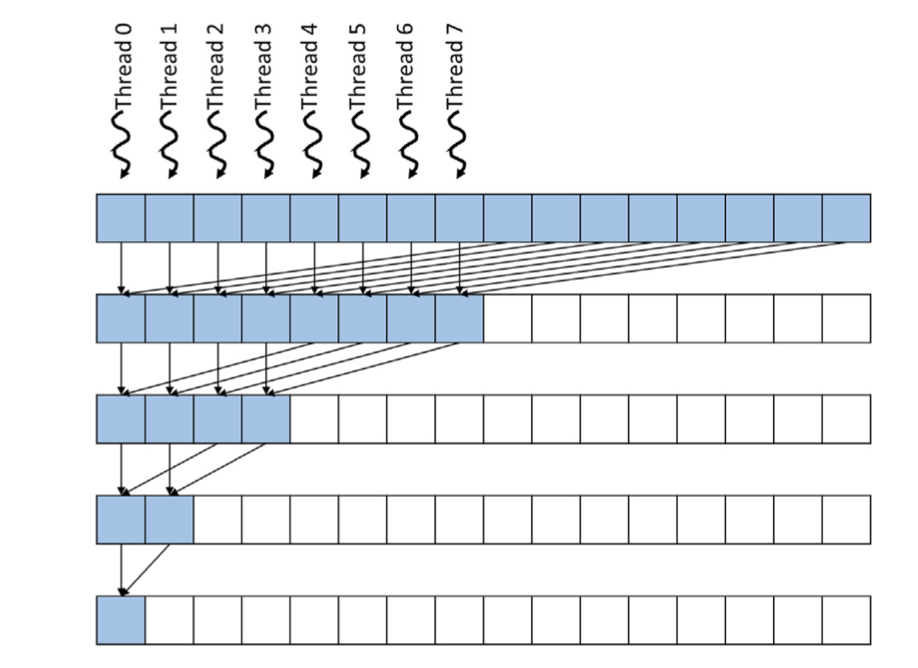
\includegraphics[width=0.9\textwidth]{figs/F10.8.png}
	\caption{\textit{使用Kernel捆绑包显式编译Kernel }}
\end{figure}

为了更好地控制Kernel编译的时间和方式,我们可以在将Kernel提交到队列之前显式请求编译Kernel包。 
当Kernel被提交到队列执行时,可以使用预编译的Kernel包。 
图 10-8 显示了如何在将任何Kernel提交到队列之前编译应用程序使用的所有Kernel,以及如何使用预编译的Kernel包。

此示例为与 SYCL 队列关联的 SYCL 上下文中的所有设备请求处于可执行状态的Kernel包,
这将导致应用程序中的任何Kernel(如果尚未处于可执行状态)进行即时编译。 
在这个具体示例中,Kernel非常短,编译不会花费很长时间,但如果有很多Kernel,或者它们更复杂,则此步骤可能会花费大量时间。 
当然,如果所有Kernel都被提前编译,或者如果所有Kernel都已经被即时编译,
则该操作实际上是免费的,因为所有Kernel都已经处于可执行状态。

\begin{figure}[H]
	\centering
	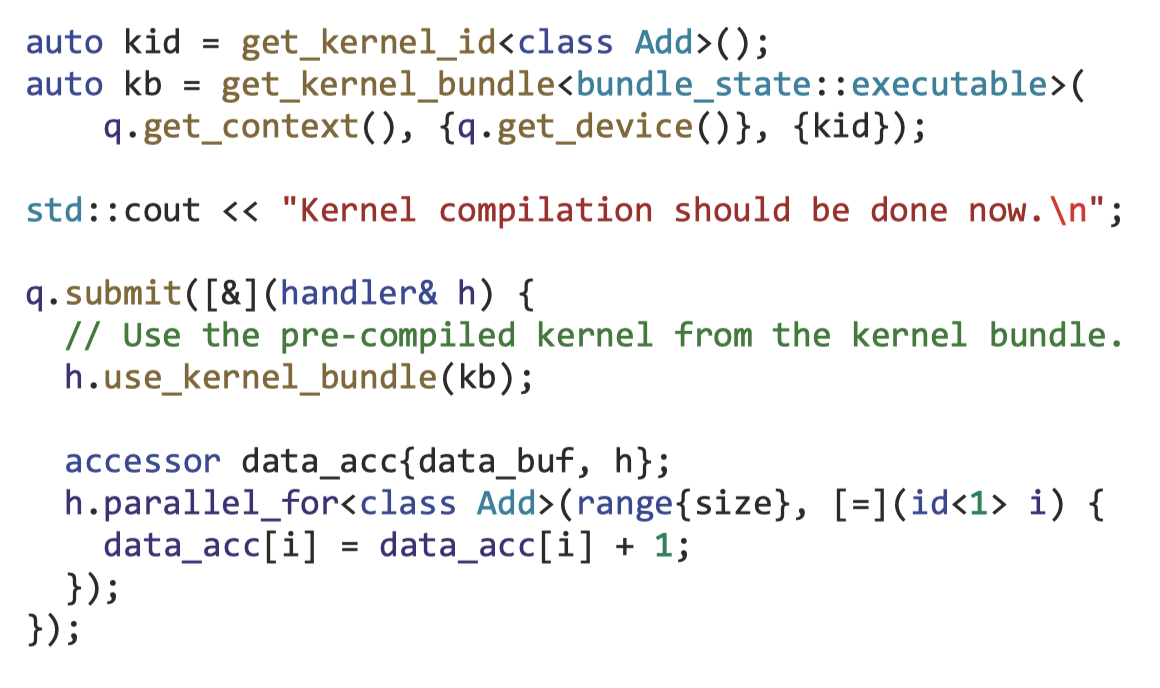
\includegraphics[width=0.9\textwidth]{figs/F10.9.png}
	\caption{\textit{使用Kernel捆绑包显式和有选择地编译Kernel }}
\end{figure}

如果我们想要更多地控制Kernel的编译时间和方式,我们可以请求特定设备的Kernel包,甚至是程序中的特定Kernel。 
这使我们能够有选择地立即编译程序中的某些Kernel,同时让其他Kernel稍后或根据需要进行编译。 
图 10-9 显示了如何仅编译由类 Add kernel name 标识的Kernel,
并且仅编译与 SYCL 队列关联的 SYCL 设备,而不是程序中的所有Kernel和 SYCL 上下文中的所有设备。

这是一种罕见的情况,我们需要命名我们的Kernel lambda 表达式; 否则,我们将无法识别要编译的Kernel。

\begin{remark}
	使用Kernel捆绑包在应用程序中以可预测的方式编译Kernel!
\end{remark}

Kernel包中的Kernel还可用于查询有关已编译Kernel的信息,例如确定特定设备的Kernel的最大工作组大小。 
在某些情况下,可能需要这些类型的Kernel查询来选择用于Kernel和特定设备的有效值。 
在其他情况下,Kernel查询可以提供提示,允许我们的应用程序动态调整并选择Kernel和特定设备的最佳值。

\begin{figure}[H]
	\centering
	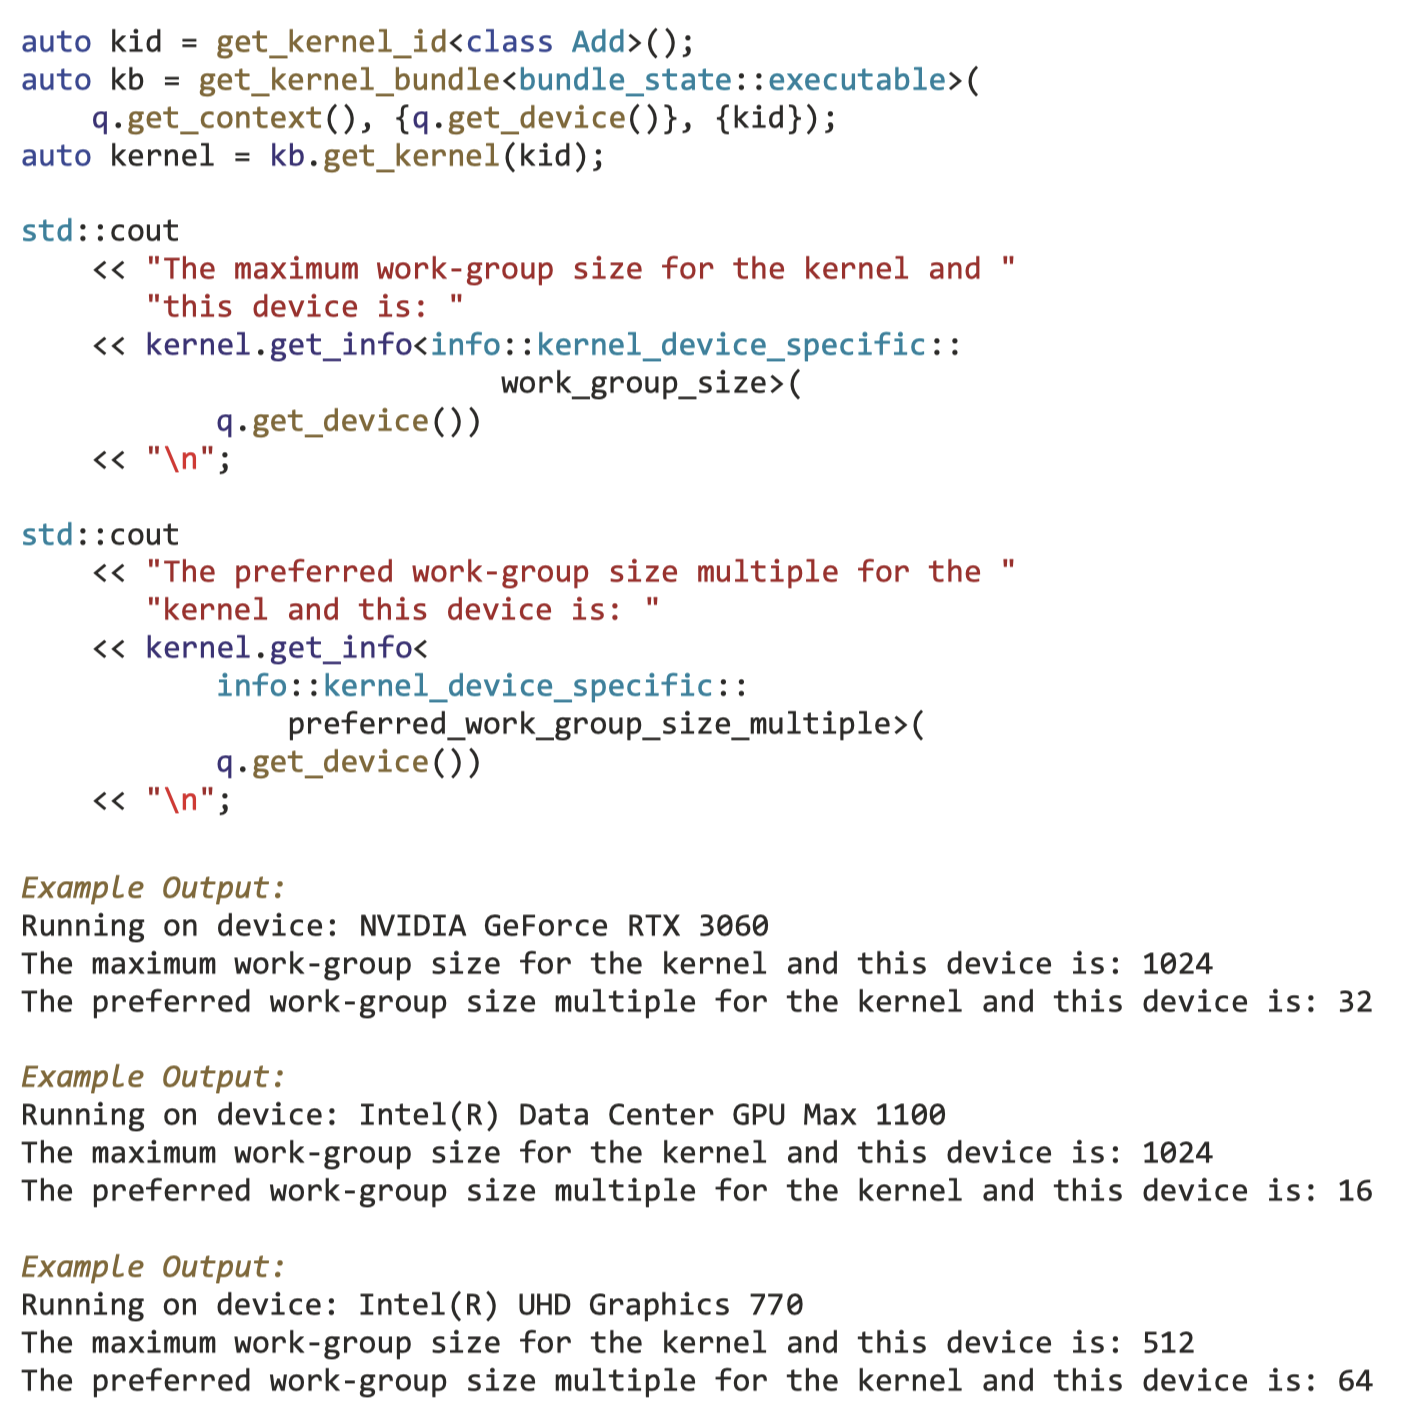
\includegraphics[width=0.9\textwidth]{figs/F10.10.png}
	\caption{\textit{查询Kernel捆绑包中的Kernel }}
\end{figure}

识别Kernel、从编译的Kernel包中获取Kernel对象以及使用Kernel对象执行设备特定查询的基本机制如图 10-10 所示。 
第 12 章描述了更完整的可用Kernel查询列表。

这是另一种罕见的情况,我们需要命名我们的Kernel lambda 表达式; 否则,我们将无法识别要查询的Kernel。

\subsection{与其他 API 的互操作性}
当 SYCL 实现构建在另一个 API 之上时,该实现可能能够与使用底层 API 机制定义的Kernel进行互操作。 
这允许应用程序轻松地将 SYCL 集成到已经使用底层 API 的现有代码库中。 
第 20 章详细介绍了这个主题。就本章而言,
我们可以简单地认识到与通过其他源语言或 API 创建的Kernel或Kernel包的互操作性提供了第三种表示Kernel的方法。

\subsection{总结}
在本章中,我们探索了定义Kernel的不同方法。 
我们描述了如何通过将Kernel表示为 C++ lambda 表达式或命名函数对象,将 SYCL 无缝集成到现有 C++ 代码库中。 
对于新的代码库,我们还讨论了不同Kernel表示的优缺点,以帮助根据应用程序或库的需求选择定义Kernel的最佳方法。

我们描述了Kernel通常如何在 SYCL 应用程序中编译,以及如何直接操作Kernel包中的Kernel来控制编译过程。 
尽管大多数应用程序不需要这种级别的控制,但在调整应用程序时,这是一种需要注意的有用技术。